\documentclass{beamer}
\usetheme{Boadilla} 
\setbeamercovered{invisible}
\setbeamertemplate{navigation symbols}{} 
%\useoutertheme{infolines} 

\usepackage[utf8]{inputenc}
\usepackage{graphicx}

\setbeamertemplate{frametitle continuation}{} 
\usepackage{subfigure}
\usepackage{caption}
\usepackage{bm}
\usepackage{epsfig}

\usepackage{amsmath}
\usepackage{xcolor,colortbl}

\usepackage{multicol}
\usepackage{wasysym}

\usepackage{hyperref}
\usepackage{float}

\usepackage{array}
\newcolumntype{L}[1]{>{\raggedright\let\newline\\\arraybackslash\hspace{0pt}}m{#1}}
\newcolumntype{C}[1]{>{\centering\let\newline\\\arraybackslash\hspace{0pt}}m{#1}}
\newcolumntype{R}[1]{>{\raggedleft\let\newline\\\arraybackslash\hspace{0pt}}m{#1}}

% deal with spaces in absolute paths

\usepackage[space]{grffile}
\graphicspath{{C:/Users/Yered/Dropbox/Harvard/Winter 2014/CdeC/Slides/Introduction/figures/}}

\usepackage[scaled]{helvet}
\usepackage[round]{natbib}


\begin{document}
\title[Introducción a la Expresión Genética]{Explorando el Transcriptoma con Datos de Expresi\'{o}n Gen\'{e}tica\\
\vspace{0.5cm}
Introducción a los Microarreglos}
\author{Yered Pita-Ju\'{a}rez}
\institute[CdeC M\'{e}rida]{}
\date{3/1/2015}


\begin{frame}
\titlepage
\end{frame}


\begin{frame}{Motivación}
\begin{itemize}
\item Dogma Central: flujo de información
\end{itemize}
\begin{figure}[H]
\centering
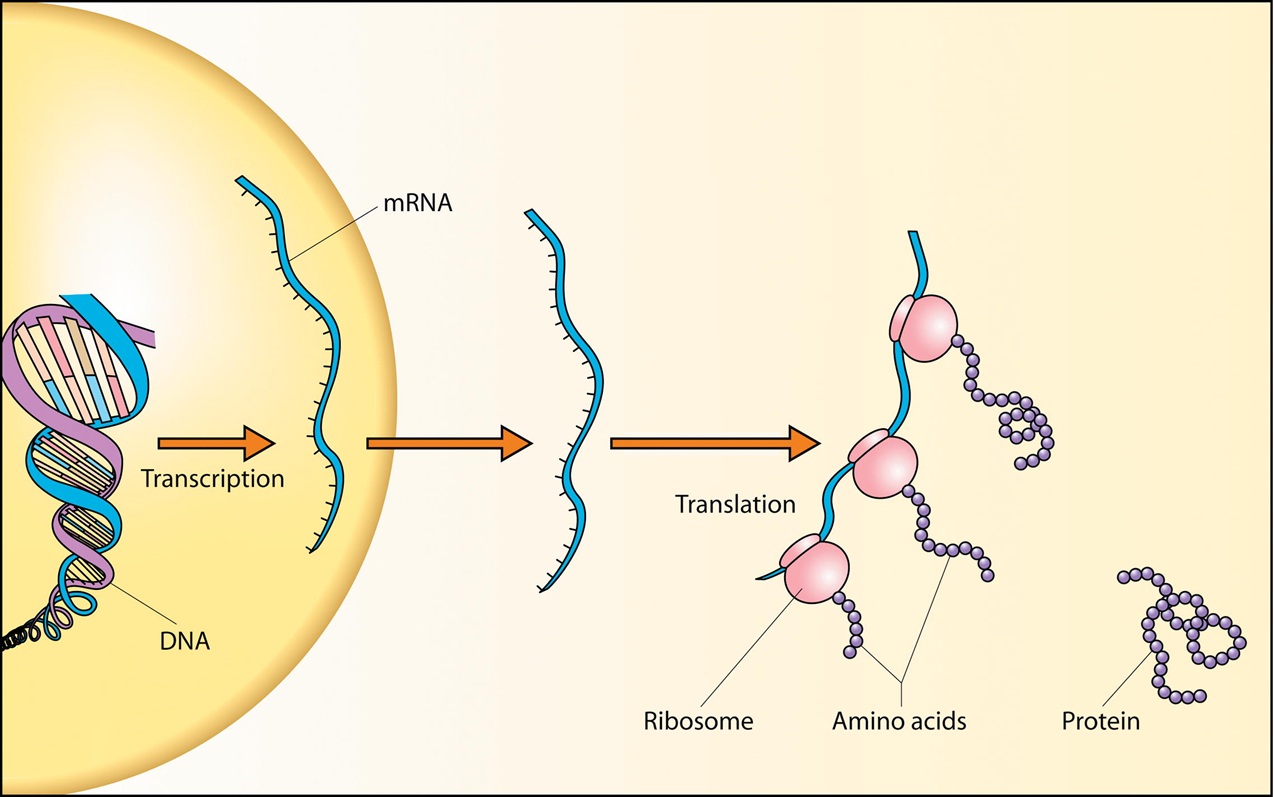
\includegraphics[scale=0.45]{dogma_diagram.png}
\end{figure}
\end{frame}



%\begin{frame}{Expresión Genética}
%\begin{itemize}
%\item Dogma Central: flujo de información
%\end{itemize}
%\begin{figure}[H]
%\centering
%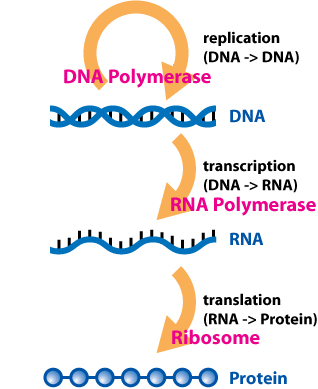
\includegraphics[scale=0.45]{central_dogma.jpg}
%\end{figure}
%\end{frame}


%\begin{frame}{Gen}
%\begin{figure}[H]
%\centering
%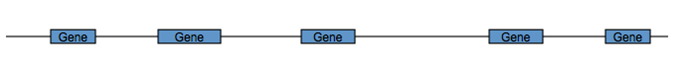
\includegraphics[scale=0.5]{gene00.png}
%\end{figure}
%\begin{figure}[H]
%\centering
%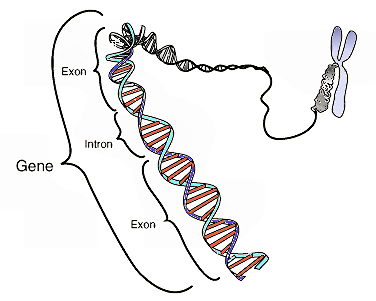
\includegraphics[scale=0.5]{gene01.png}
%\end{figure}
%\end{frame}
%
%\begin{frame}{Transcripción}
%\begin{figure}[H]
%\centering
%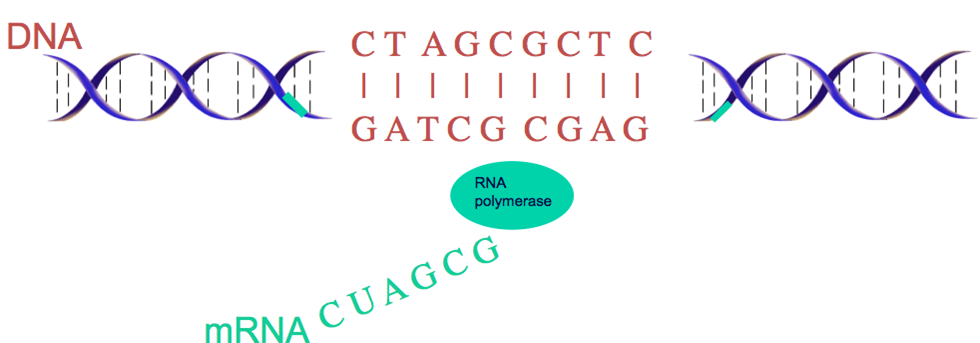
\includegraphics[scale=0.45]{gene02.png}
%\end{figure}
%\end{frame}
%
%\begin{frame}{Traducción}
%\begin{figure}[H]
%\centering
%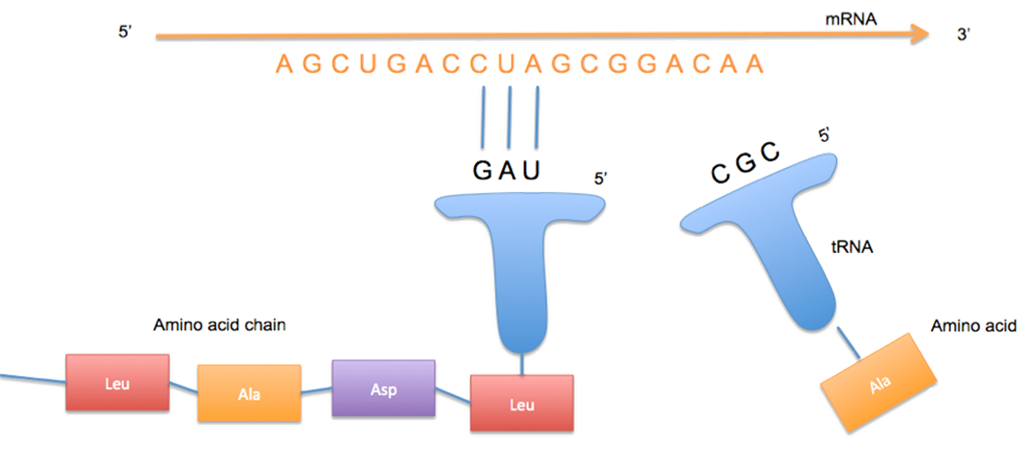
\includegraphics[scale=0.45]{gene03.png}
%\end{figure}
%\end{frame}

\begin{frame}{Transcriptoma}
\begin{itemize}
\item El conjunto de todas las moleculas de ARN en las células
\item Una célula no requiere de todas las proteínas, y las que usa las requiere en diferentes cantidades
%\item Expresión genética 
%\begin{itemize}
%	\item Expresión baja: produciendo pocas o nada de proteínas
%	\item Expresión alta: produciendo proteínas en abundancia
%\end{itemize}
%\item Medir niveles de ARN: expresión genética
\end{itemize}
\begin{figure}[H]
\centering
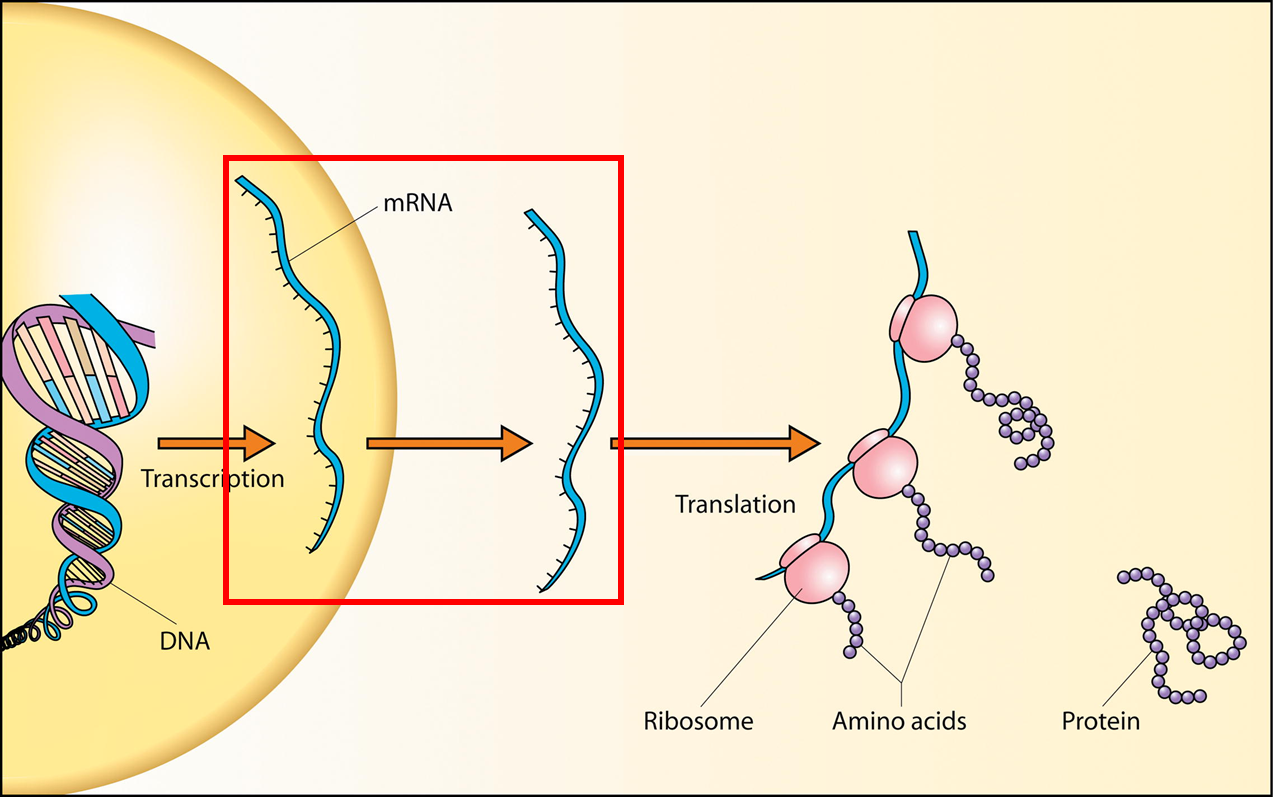
\includegraphics[scale=0.35]{transcriptome.png}
\end{figure}
\end{frame}

\begin{frame}{Transcriptoma}
\begin{itemize}
%\item El conjunto de todas las moleculas de ARN en las células
%\item Una célula no requiere de todas las proteínas, y las que usa las requiere en diferentes cantidades
\item Expresión genética 
\begin{itemize}
	\item Expresión baja: produciendo pocas o nada de ARN
	\item Expresión alta: produciendo ARN en abundancia
\end{itemize}
\item Medir niveles de ARN: expresión genética
\end{itemize}
\begin{figure}[H]
\centering
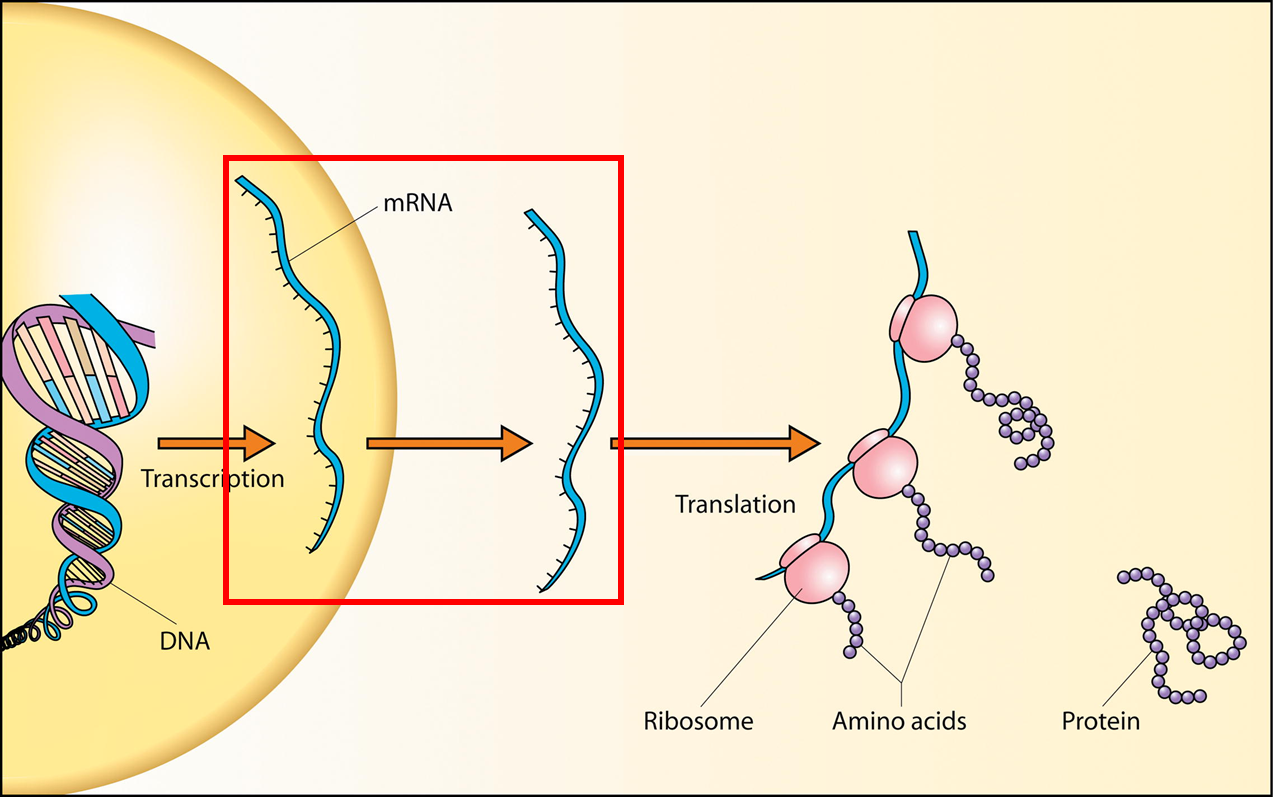
\includegraphics[scale=0.35]{transcriptome.png}
\end{figure}
\end{frame}


\begin{frame}{Microarreglos}
\begin{itemize}
\item Microarreglos: contar moleculas de ARN
\item Requiere MUCHAS moleculas de ARN
\item El ARN proviene de un conjunto de células
\end{itemize}
\begin{figure}[H]	
\centering
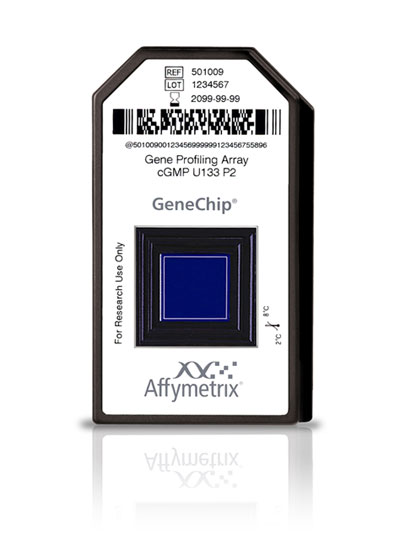
\includegraphics[scale=0.25]{gene_profile_array_large.jpg}
\end{figure}
\end{frame}



\begin{frame}{Desnaturalización}
\begin{itemize}
\item Separar el ADN en una sola cadena
\end{itemize}
\begin{figure}[H]
\centering
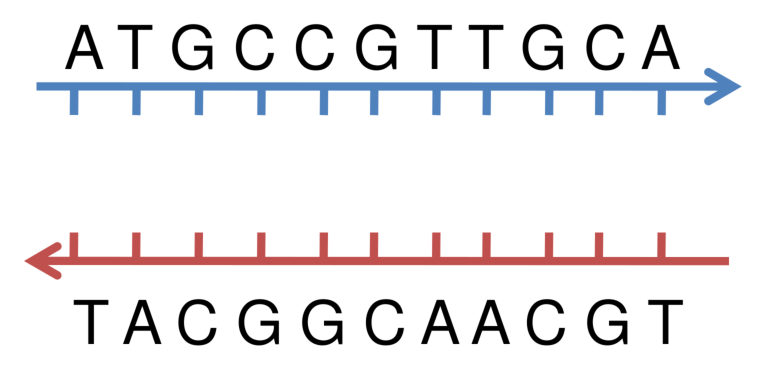
\includegraphics[scale=0.55]{denaturation.pdf}
\end{figure}
\end{frame}

\begin{frame}{Hibridación}
\begin{itemize}
\item Una cadena de ADN se una a su complemento
\end{itemize}
\begin{figure}[H]
\centering
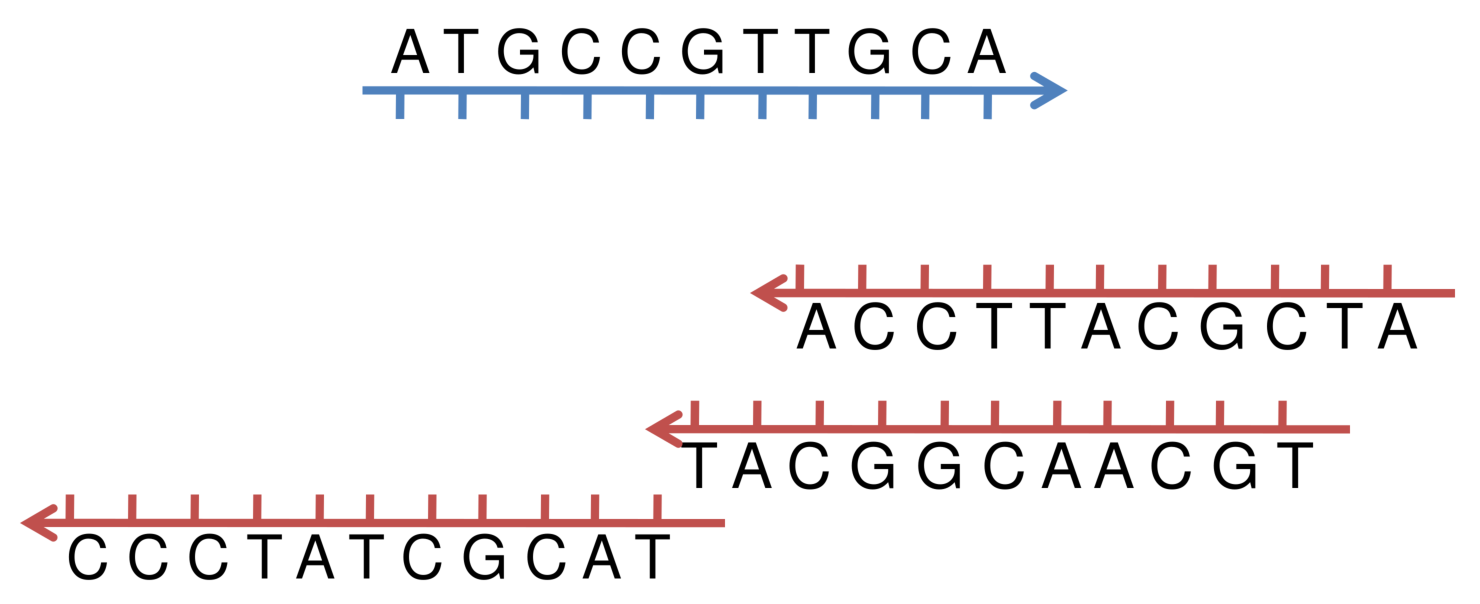
\includegraphics[scale=0.45]{hybridization00.pdf}
\end{figure}
\end{frame}


\begin{frame}{Hibridación}
\begin{itemize}
\item Una cadena de ADN se una a su complemento
\end{itemize}
\begin{figure}[H]
\centering
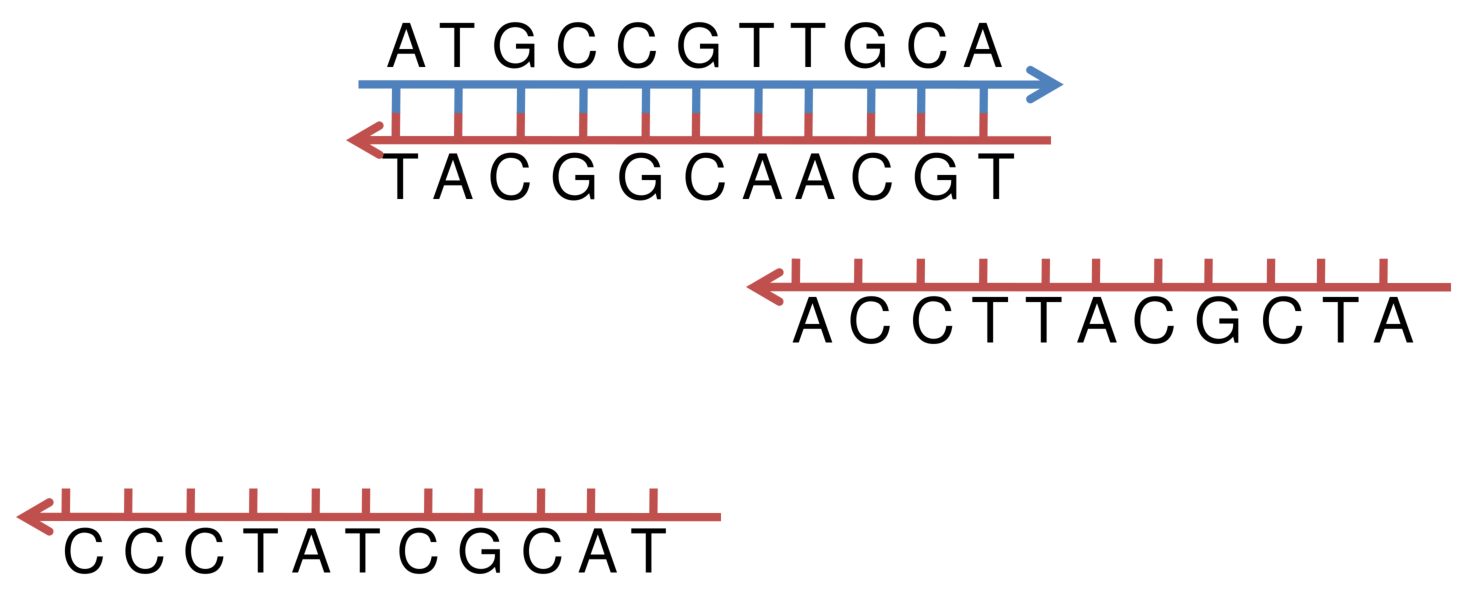
\includegraphics[scale=0.45]{hybridization01.pdf}
\end{figure}
\end{frame}


%\begin{frame}{Microarreglos}
%\begin{figure}
%\centering
%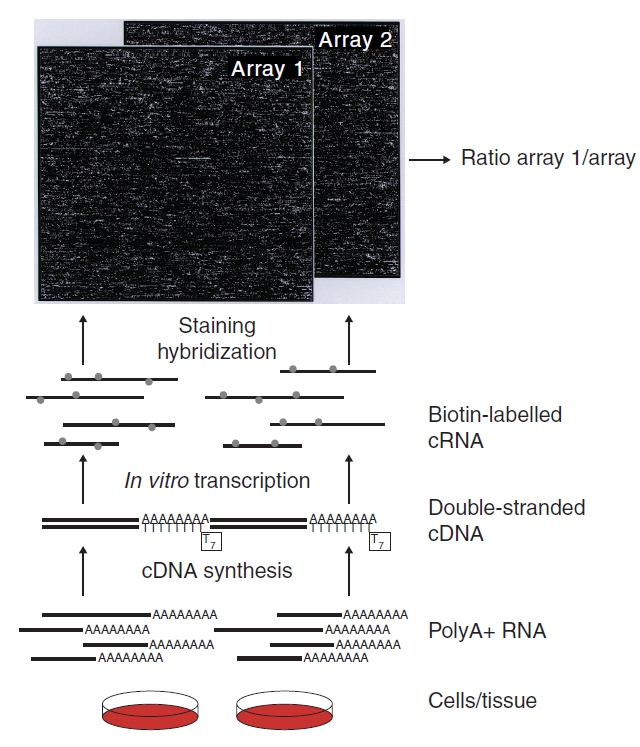
\includegraphics[scale=0.4]{microarray_diagram}
%\end{figure}
%\end{frame}

\begin{frame}{Sondas}
\begin{itemize}
\item Sonda: cadenas de ADN complementarias
\item las sondas se diseñan a partir de una secuencia conocida
\item Ejemplo: 4 sondas con 4 replicados cada una
\end{itemize}
\begin{figure}[H]
\centering
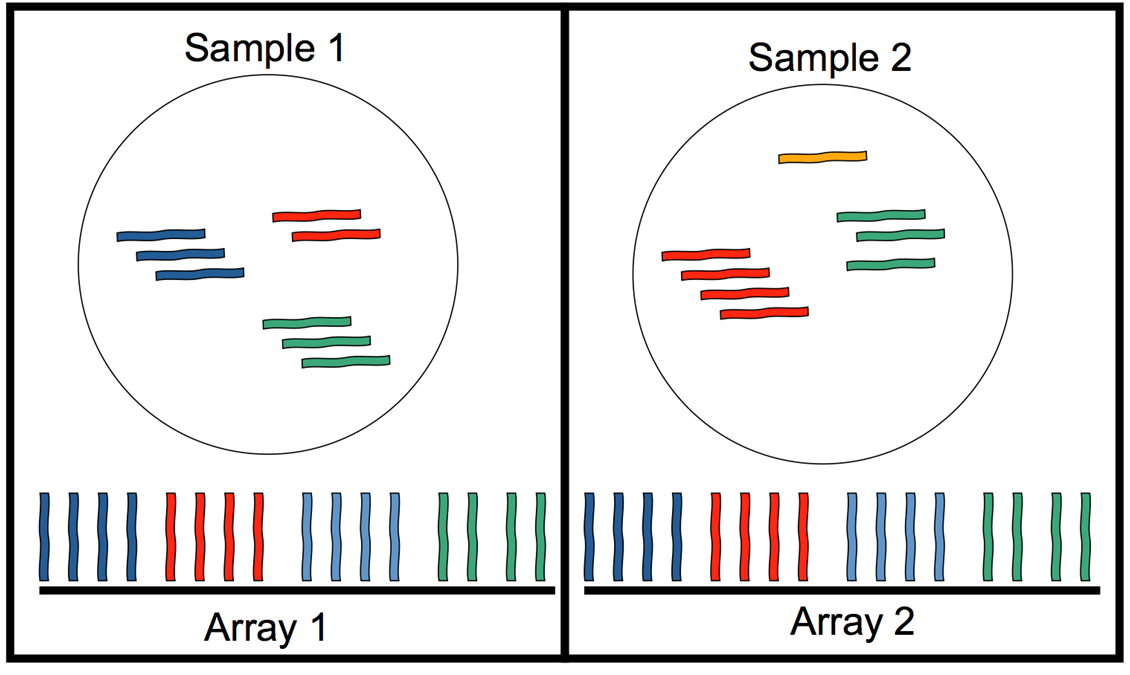
\includegraphics[scale=0.45]{probes.png}
\end{figure}
\end{frame}


\begin{frame}{Etiquetado}
\begin{itemize}
\item Distinguir a las secuencias
\item Etiqueta: tinte agregado a las secuencias
\item Hibridación con las sondas
\end{itemize}
\begin{figure}[H]
\centering
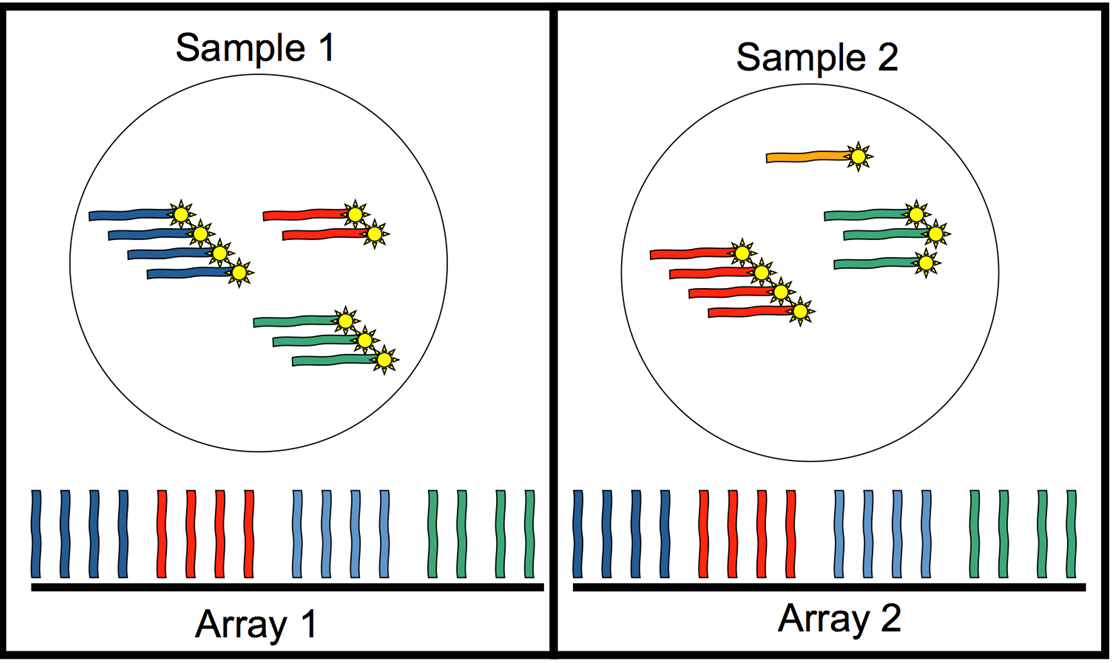
\includegraphics[scale=0.45]{labeling.png}
\end{figure}
\end{frame}

\begin{frame}{Etiquetado}
\begin{itemize}
\item Distinguir a las secuencias
\item Etiqueta: tinte agregado a las secuencias
\item Hibridación con las sondas
\end{itemize}
\begin{figure}[H]
\centering
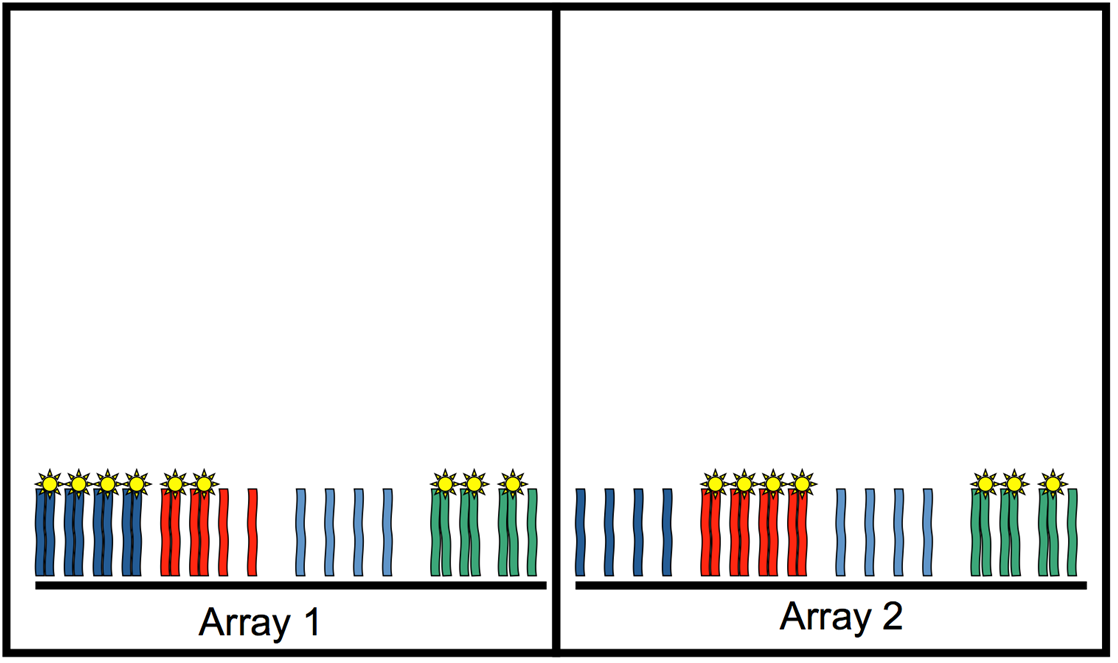
\includegraphics[scale=0.45]{post_hybridization.png}
\end{figure}
\end{frame}

\begin{frame}{Post-Hibridación}
\begin{itemize}
\item Intensidad del tinte proporcional a la cantidad de secuencias capturadas
\item $\uparrow$ intensidad : $\uparrow$ secuencias hibridizadas
\end{itemize}
\begin{figure}[H]
\centering
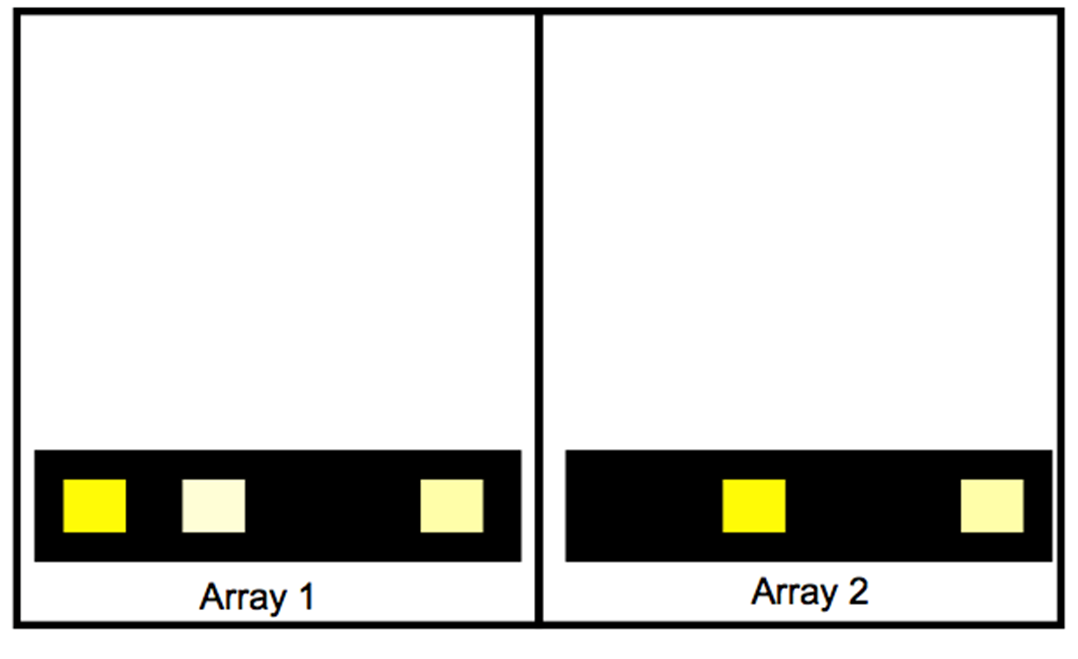
\includegraphics[scale=0.45]{scanner.png}
\end{figure}
\end{frame}

\begin{frame}{Cuantificación}
\begin{itemize}
\item Un escáner mide fotones: intensidades 
\end{itemize}
\begin{figure}[H]
\centering
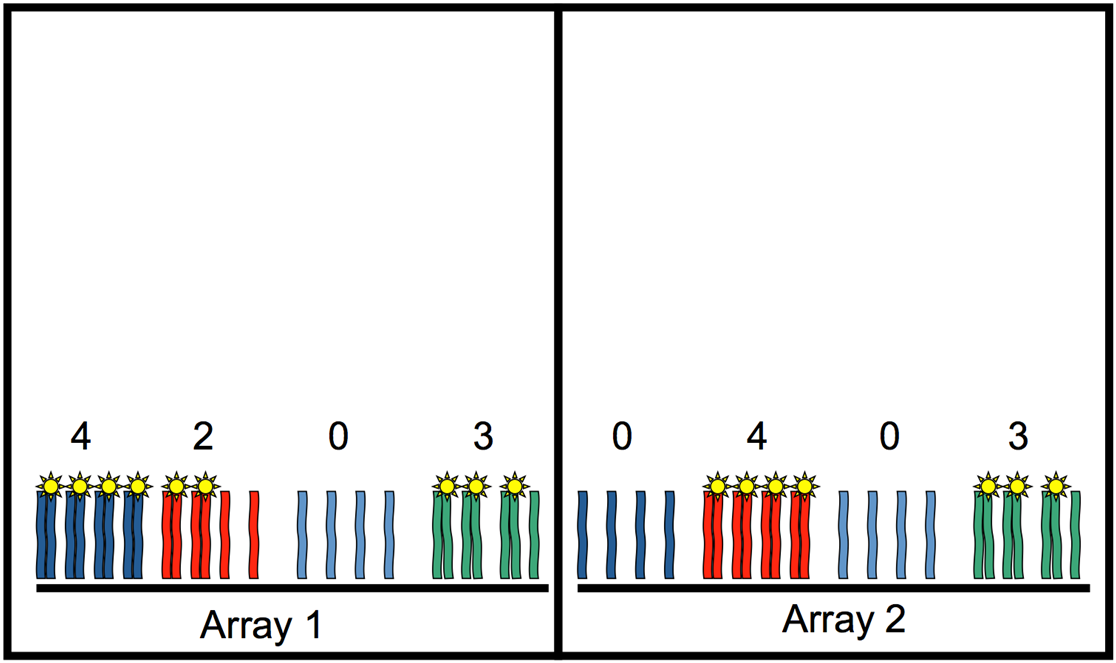
\includegraphics[scale=0.45]{quantification.png}
\end{figure}
\end{frame}

\begin{frame}{Microarreglo}
\begin{figure}[H]
\centering
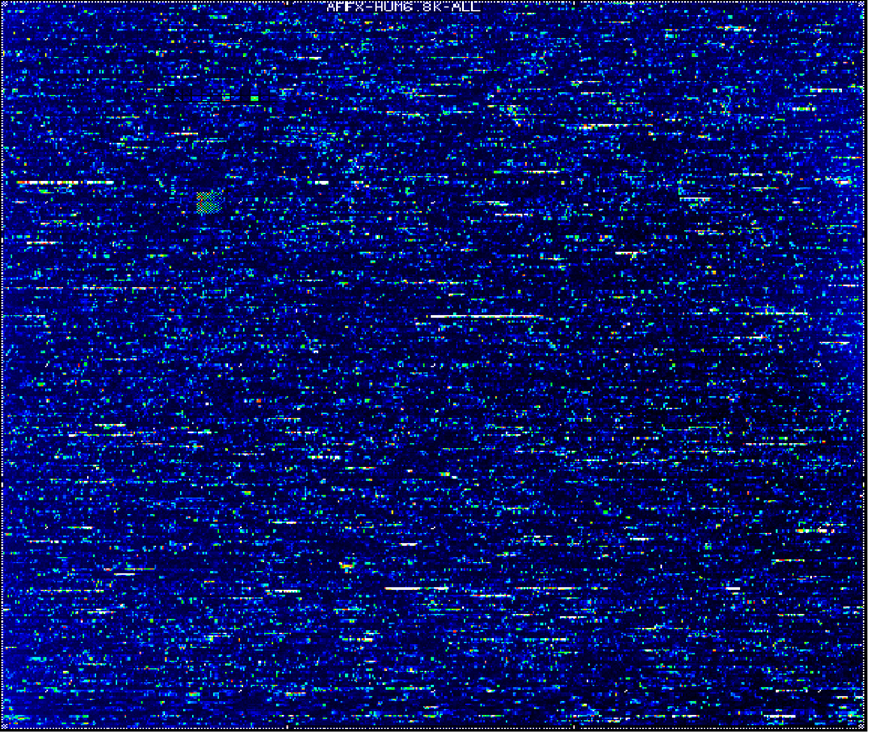
\includegraphics[scale=0.4]{actual_microarray.png}
\end{figure}
\begin{itemize}
\item Miles de sondas
\item Cada cuadro es una sonda con diferente intensidad
\end{itemize}
\end{frame}

%\begin{frame}{Affymetrix}
%\begin{figure}
%\centering
%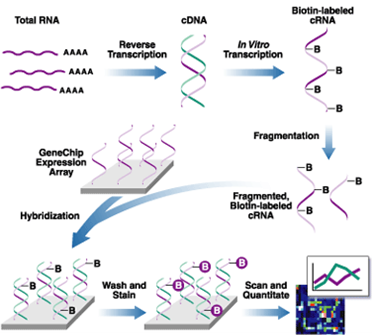
\includegraphics[scale=0.45]{affy_overview.png}
%\end{figure}
%\end{frame}


\begin{frame}{Affymetrix}
\begin{itemize}
\item Divido en miles de celdas
\item Cada celda contiene varias sondas
\item Cada sonda contiene varias cadenas de 25 bases
\end{itemize}
\begin{figure}[H]
\centering
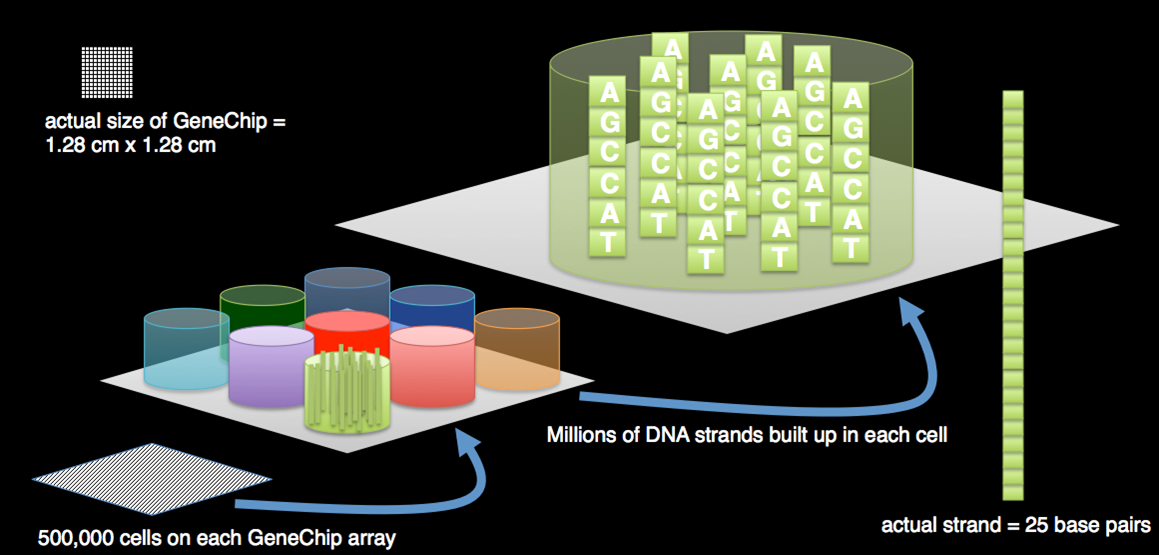
\includegraphics[scale=0.45]{affy00.png}
\end{figure}
\end{frame}

\begin{frame}{Affymetrix}
\begin{itemize}
\item Secuencias etiquetadas
\item Las secuencias se hibridizan en el microarreglo
\item Cada sonda es específica a una secuencia particular
\end{itemize}
\begin{figure}[H]
\centering
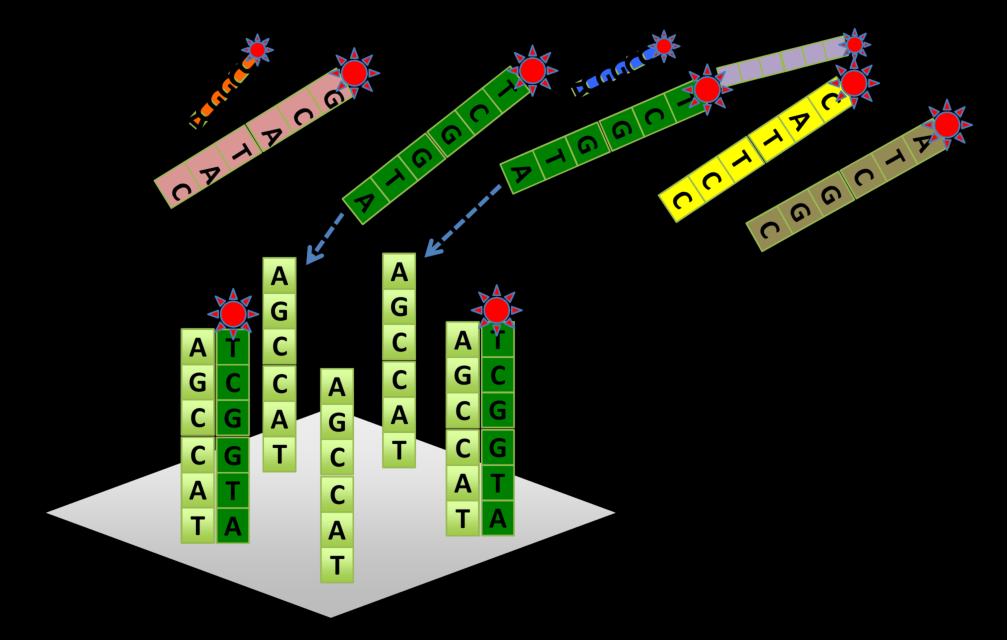
\includegraphics[scale=0.45]{affy01.pdf}
\end{figure}
\end{frame}

\begin{frame}
\begin{figure}[H]
\centering
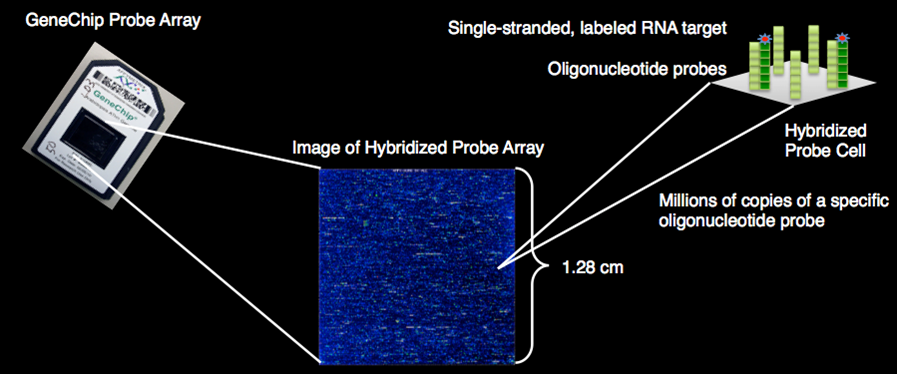
\includegraphics[scale=0.45]{affy02.png}
\end{figure}
\end{frame}

\begin{frame}
\begin{figure}[H]
\centering
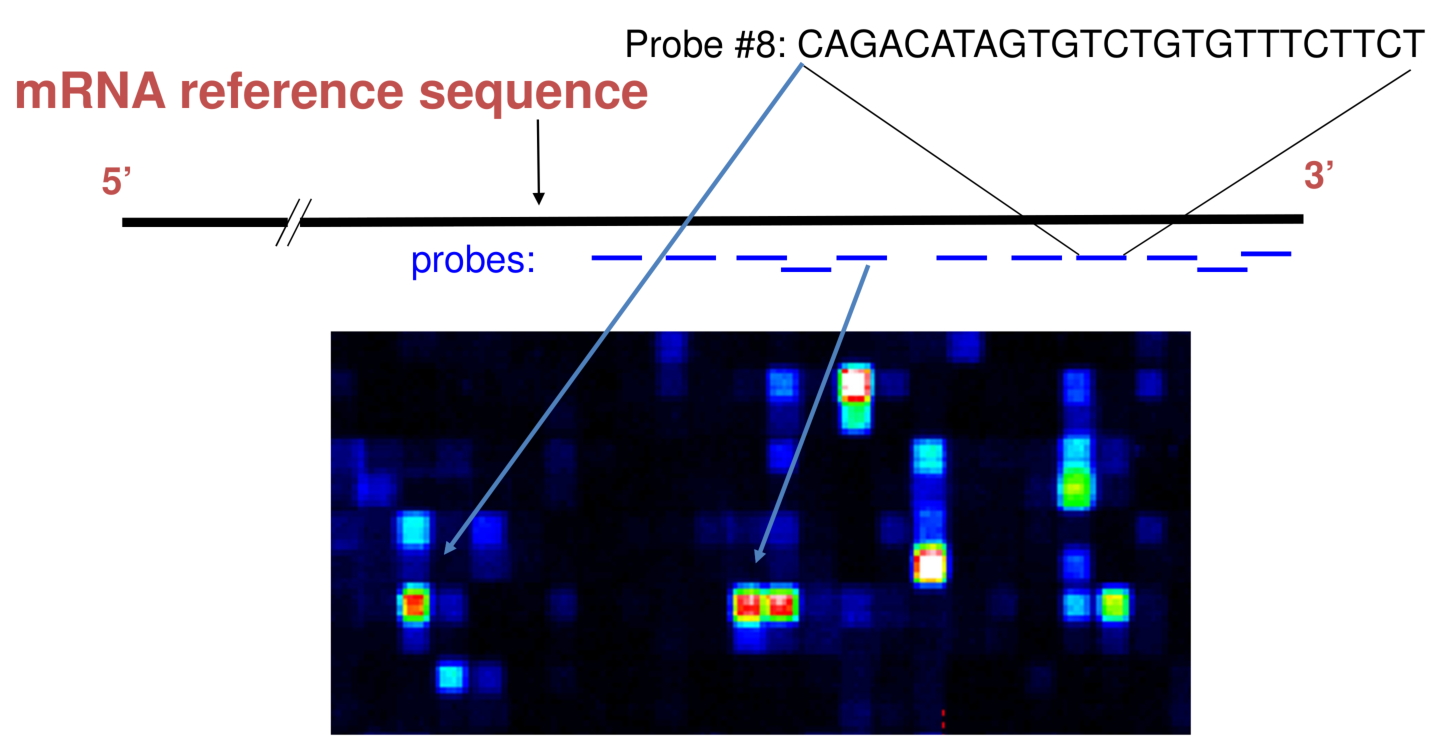
\includegraphics[scale=0.45]{affy_gene_exp.pdf}
\end{figure}
\end{frame}


\end{document} 

%\begin{frame}{Microarreglos}
%\begin{figure}
%\centering
%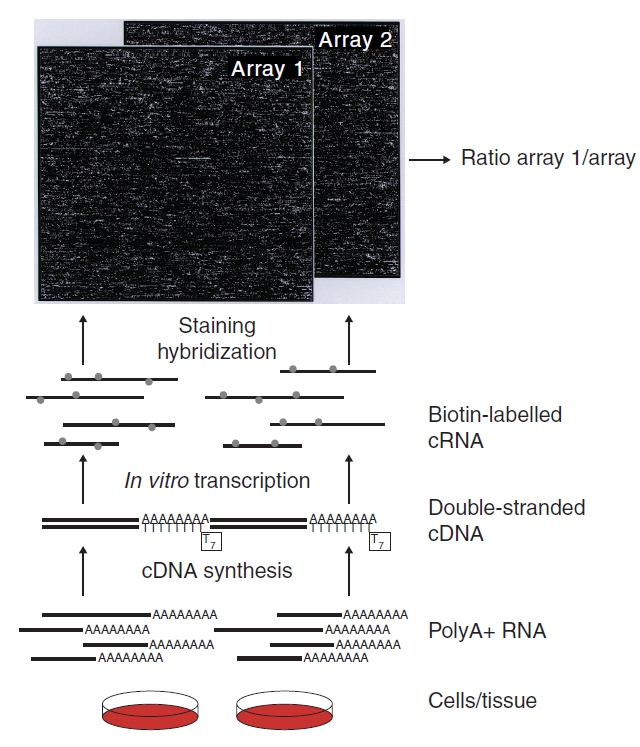
\includegraphics[scale=0.4]{microarray_diagram}
%\end{figure}
%\end{frame}

%\begin{frame}{Affymetrix}
%\begin{figure}
%\centering
%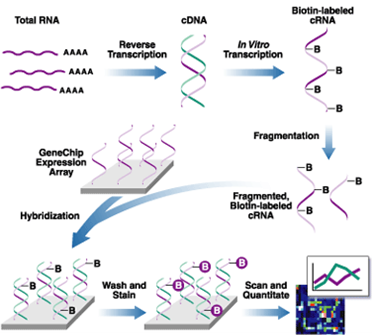
\includegraphics[scale=0.45]{affy_overview.png}
%\end{figure}
%\end{frame}
